\documentclass[11pt,a4paper]{article}
\usepackage[utf8]{inputenc}
\usepackage[T1]{fontenc}
\usepackage[brazilian]{babel}
\usepackage[margin=2.3cm]{geometry}
\usepackage{graphicx}
\usepackage{booktabs}
\usepackage{array}
\usepackage{xcolor}
\usepackage{hyperref}
\usepackage{caption}
\usepackage{amsmath}
\usepackage{longtable}
\usepackage{float}
\usepackage{enumitem}
\usepackage{multirow}

\hypersetup{
  colorlinks=true,
  linkcolor=blue!50!black,
  urlcolor=blue!50!black,
  citecolor=blue!50!black
}

\title{Reproduzindo a Política de Detecção do Francisco\\
\large Metodologia passo a passo, portada para a nossa pipeline, e o resultado
de tentar bater o mesmo número de falso positivo}
\author{Pipeline \texttt{cnn1d\_ae} / AutoML --- projeto \texttt{TesteMLCab}\\
\small Branch \texttt{AE\_pca\_monitoramento\_sistema}}
\date{Agosto de 2026}

\begin{document}
\maketitle

\begin{abstract}
Um colega do projeto (Francisco), trabalhando na branch
\texttt{feat/pdm-deteccao-4sinais}, construiu um detector de anomalias
para a mesma turbina que reporta \textbf{0,94 falsos positivos por mês}
com \textbf{6 de 8 falhas reais detectadas} --- um resultado bem melhor
que o obtido até então pela nossa abordagem de PCA sobre todos os
sensores (3,35--5,77 FP/mês). Em vez de assumir que a diferença vinha de
um modelo melhor, lemos o código dele (sem executá-lo) e identificamos
nove decisões de engenharia concretas por trás desse número. Este
relatório descreve essas decisões passo a passo e documenta a tentativa
de portá-las para a nossa própria pipeline (pré-processamento real do
projeto, \texttt{scikit-learn} puro) --- não para copiar o código dele,
mas para testar se o \emph{mecanismo} se sustenta fora do código original
dele. Resultado: o falso positivo foi replicado quase exatamente
(\textbf{0,90 FP/mês} contra os 0,94/mês dele), confirmando que a
supressão de falso positivo vem da arquitetura de confirmação entre
sinais independentes, não de um modelo ponto a ponto mais preciso. A
cobertura de eventos, porém, ficou bem abaixo da dele (2 de 11 eventos
curados no nosso dataset, contra 6 de 8 no dele) --- gap registrado como
próximo passo, com uma hipótese concreta já identificada.
\end{abstract}

\tableofcontents

% =====================================================================
\section{Contexto: de onde veio a comparação}
% =====================================================================

Desde o EXP10c (autoencoder dedicado ao sensor T5), o projeto vinha
construindo pipelines de detecção \emph{por alvo}: escolher um
sensor/alarme, treinar um modelo específico para ele. Para explorar uma
abordagem complementar --- um único modelo vigiando a planta inteira,
sem escolher um alvo --- construímos uma série de experimentos de PCA
com retreino mensal (\texttt{scripts/pca\_monitoramento\_sistema/},
v1 a v4), avaliados contra o catálogo completo de 47 tags de alarme.

Nesse processo, uma pergunta levantada pelo usuário --- ``será que os
alarmes de um mesmo equipamento disparam todos juntos quando há uma
falha de verdade?'' --- levou a uma checagem empírica que confirmou um
\emph{efeito cascata}: até 46 dos 47 tags do catálogo disparam dentro de
minutos um do outro no mesmo evento físico. Isso, por sua vez, levantou
a suspeita de que nossa métrica de falso positivo (calculada por tag,
contra o catálogo bruto) poderia não ser comparável a métricas externas.

Uma imagem trazida pelo usuário mostrou o resultado de um colega
(Francisco) na branch \texttt{feat/pdm-deteccao-4sinais}, reportando
\textbf{0,94 falsos positivos por mês} --- uma unidade (episódios/mês)
diferente da nossa (\% de pontos), mas comparável depois de convertida.
Isso motivou a leitura completa do código e da documentação dele para
entender \emph{como} ele chega nesse número, e a tentativa de reproduzir
o mecanismo por trás dele --- não como benchmark oficial (os datasets e
períodos avaliados diferem), mas como validação de que entendemos
corretamente por que a diferença existe.

% =====================================================================
\section{A metodologia do Francisco, passo a passo}
% =====================================================================

Toda esta seção descreve decisões de engenharia dele, lidas diretamente
de \texttt{README\_PDM.md}, \texttt{src/cabiunas\_pdm/config.py} e
\texttt{scripts/automl\_clearml.py} na branch \texttt{feat/pdm-deteccao-4sinais}
(leitura remota via \texttt{git show}, sem \texttt{checkout} nem execução
do código dele). A Figura~\ref{fig:pipeline} resume o fluxo da política
de produção final dele (\texttt{DETECTION\_POLICY}, decisão de
18/07/2026, prioridade explícita ``minimizar falso positivo'').

\begin{figure}[H]
\centering
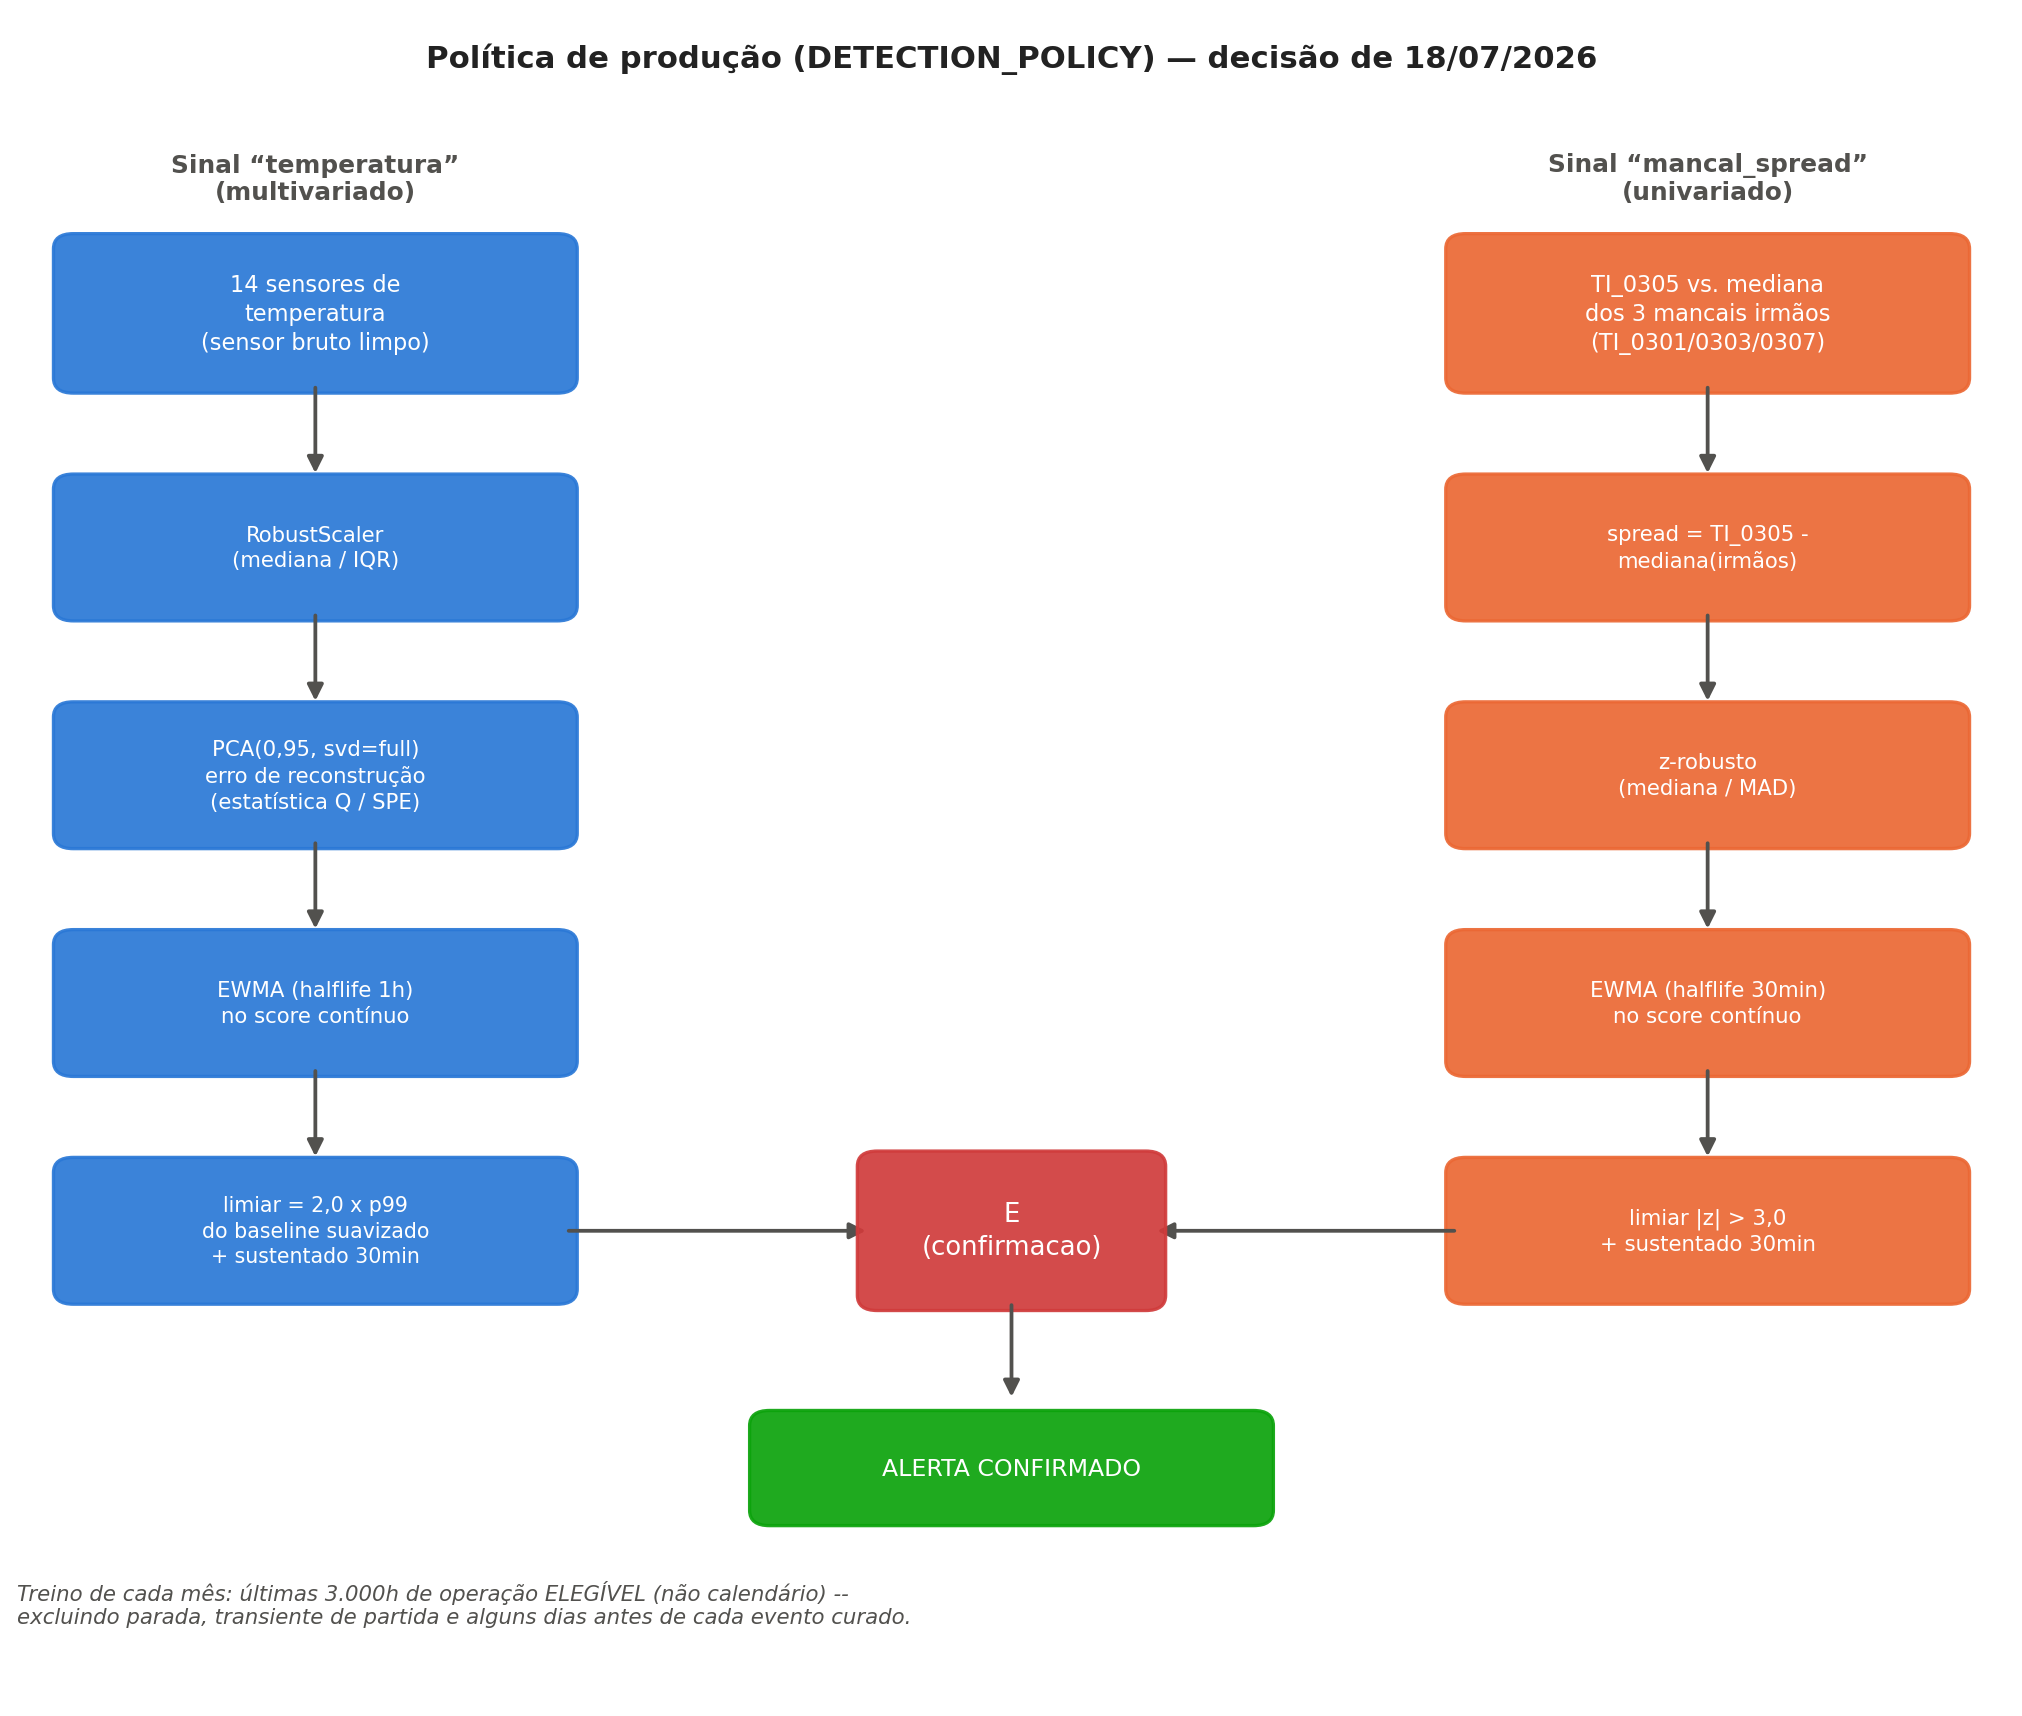
\includegraphics[width=0.92\textwidth]{fig_pipeline_v6.png}
\caption{Fluxo da política de produção do Francisco: dois sinais
independentes (temperatura multivariada e spread de mancal univariado),
cada um com seu próprio pré-processamento, suavização e limiar, exigindo
confirmação simultânea (E lógico) para emitir um alerta.}
\label{fig:pipeline}
\end{figure}

\subsection{Quatro sinais, agrupados por subsistema físico --- não um
PCA único sobre todos os sensores}

A diferença conceitual mais importante: em vez de um único modelo
recebendo os $\sim$36 sensores brutos juntos (nossa abordagem v1--v4),
ele decompõe o problema em \textbf{quatro sinais independentes},
alinhados aos mecanismos de falha conhecidos do equipamento:

\begin{itemize}[leftmargin=1.4em]
  \item \textbf{\texttt{temperatura}} --- multivariado, 14 sensores de
  temperatura/exaustão (os mesmos termopares \texttt{TC382\_0X\_A},
  \texttt{TI\_03XX} e \texttt{T5\_AVG\_A} que já usamos).
  \item \textbf{\texttt{pressao\_oleo}} --- multivariado, 12 sensores de
  pressão/óleo/selagem.
  \item \textbf{\texttt{mancal\_spread}} --- univariado: \texttt{TI\_0305}
  menos a mediana dos 3 mancais irmãos (\texttt{TI\_0301}/\texttt{0303}/\texttt{0307}).
  \item \textbf{\texttt{selagem\_z}} --- univariado: \texttt{PDIT\_0305}
  isolado.
\end{itemize}

Os dois sinais univariados existem por uma medição concreta dele,
documentada no código: abrindo o erro de reconstrução por sensor antes
da falha de selagem de 27/02/2025, o \texttt{PDIT\_0305} respondia por
53\% do erro total --- e mesmo assim não gerou alerta, porque o score da
família de pressão é a \emph{média} sobre 12 sensores, e um sensor
gritando vira sussurro depois de dividido por 12. Isolar esse sensor
específico como sinal próprio resolve essa diluição. O mesmo raciocínio
motivou o \texttt{mancal\_spread}: comparar um mancal contra os irmãos
físicos (redundantes por construção) é mais sensível a uma falha
\emph{localizada} do que qualquer estatística agregada da família
inteira.

Vibração fica de fora dos quatro sinais (``quarentena''), porque o
normal dela deriva ao longo dos meses sem falha associada --- o mesmo
achado que já tínhamos documentado na nossa própria investigação
(Seção~\ref{sec:interpretacao}).

\subsection{Ground-truth curado, não o catálogo bruto de alarmes}
\label{sec:ground-truth}

Diferença metodológica central: ele \textbf{não avalia contra os 3757
eventos \texttt{ACT} do catálogo}. Deriva uma lista curta de
\emph{trips reais} com um algoritmo objetivo, em três passos:

\begin{enumerate}[leftmargin=1.6em]
  \item \textbf{Parada real} = transição \texttt{RUNNING\_A} $1\to0$ que
  dura $\geq$ 2 horas (abaixo disso é queda de telemetria, não parada de
  máquina --- medido por ele: 65 das 135 transições da grade de 30s
  duram menos de 3 minutos).
  \item \textbf{Trip} = parada real \emph{coincidente} com um alarme de
  \emph{nível} (texto da descrição casando o padrão
  \texttt{TRIP|MT.ALTA|M.ALTA|MT.BX|M.BX|MT.BAIXA|M.BAIXA}) na janela de
  $-1$h a $+30$min ao redor do início da parada. A conjunção é
  indispensável: um único tag de nível pode disparar dezenas de vezes,
  mas só uma fração pequena coincide com a máquina realmente caindo ---
  as demais são eco de uma parada que já aconteceu por outro motivo, não
  sintoma da causa raiz.
  \item \textbf{Evento físico} = trips a menos de 24h um do outro,
  agrupados e contados uma única vez (evita contar a mesma falha
  duas vezes quando ela dispara mais de um trip em sequência).
\end{enumerate}

Esse algoritmo produziu \textbf{8 eventos físicos} no período avaliado
por ele (jan/2025 a abr/2026). A mesma lógica, replicada no
Seção~\ref{sec:eventos-curados} sobre o nosso dataset, produz 11 eventos
num período mais longo (mar/2024 a abr/2026).

\subsection{PCA-Q (erro de reconstrução), não PCA + \texttt{iforest}}

Para o sinal \texttt{temperatura} (e \texttt{pressao\_oleo}), ele usa
\texttt{PCA(n\_components=0{,}95, svd\_solver="full")} --- deixando o
próprio \texttt{scikit-learn} escolher quantos componentes bastam para
explicar 95\% da variância, em vez de fixar um número de componentes a
priori. O score é o erro quadrático médio entre a entrada normalizada e
sua reconstrução via PCA (a estatística $Q$/SPE clássica de monitoramento
de processo multivariado):
\[
  Q = \frac{1}{d}\sum_{j=1}^{d} \left(x_j - \hat{x}_j\right)^2,
  \qquad \hat{x} = W W^\top x
\]
onde $W$ são os componentes principais aprendidos no baseline. Isso é
mais simples que a nossa abordagem original (PCA para redução de
dimensionalidade, seguido de \texttt{IsolationForest} ou \texttt{OneClassSVM}
no espaço latente) --- e evita de forma elegante um bug que encontramos
na nossa própria pipeline: fixamos um teto de 20 componentes que travava
antes de atingir a meta de 90\% de variância (documentado no v2--v4,
Seção~\ref{sec:interpretacao}).

\subsection{Normalização robusta (mediana/IQR), não z-score}

Antes do PCA, ele normaliza com \texttt{RobustScaler} (centraliza pela
mediana, escala pelo intervalo interquartil), não pela média/desvio-padrão
como o nosso \texttt{NORMALIZE\_MODE="zscore"} original. A vantagem prática:
outliers extremos (picos de sensor, ruído de instrumentação) não distorcem
a escala aprendida, porque mediana e IQR são estatísticas robustas a
valores extremos --- a média e o desvio-padrão, não.

\subsection{EWMA no score contínuo, antes do limiar --- não debounce no
flag binário depois}
\label{sec:ewma}

Esta é, na nossa leitura, a decisão mais subestimada do conjunto. Nas
nossas pipelines (v1--v5), o fluxo é: calcular o erro do modelo ponto a
ponto $\to$ comparar com o limiar $\to$ obter um flag binário (0/1)
$\to$ suavizar esse flag binário (debounce, exigindo que fique ligado por
$N$ pontos seguidos). Ele inverte a ordem: suaviza o \textbf{score
contínuo} primeiro, com uma média móvel exponencial baseada em tempo
real (não em contagem de amostras),
\[
  s_t = \alpha \, e_t + (1-\alpha)\, s_{t-1}, \qquad
  \alpha = 1 - 2^{-\Delta t / h},
\]
onde $h$ é a meia-vida (\texttt{halflife}, 1h para \texttt{temperatura},
30min para \texttt{mancal\_spread}) e $\Delta t$ o intervalo real entre
amostras (relevante porque a grade não é perfeitamente regular). Só
\emph{depois} disso o limiar é aplicado. Suavizar o score contínuo antes
do corte binário produz uma curva muito menos ruidosa: um pico isolado de
1--2 amostras, que dispararia nosso flag binário instantaneamente, pode
nunca cruzar o limiar depois de passado pela EWMA --- porque o "peso"
dele na média é pequeno frente ao histórico recente.

\subsection{Limiar: múltiplo do p99 (multivariado) ou z-robusto
(univariado)}

Para o sinal \texttt{temperatura}: limiar $= 2{,}0 \times p_{99}$ do
score suavizado do próprio baseline (não $p_{99}$ diretamente --- o
fator 2 dá margem adicional). Para \texttt{mancal\_spread}: $|z| > 3{,}0$,
onde $z$ é calculado de forma robusta (mediana e MAD do baseline
suavizado, não média/desvio-padrão). Ambos exigem \textbf{sustentação de
30 minutos} --- o flag precisa ficar acima do limiar continuamente por
30 minutos (60 amostras a 30s de cadência) antes de contar.

Vale registrar uma alternativa que ele também implementou mas não usa na
política final: limiar por \emph{k-ésimo maior} valor do baseline, em
vez de percentil. A motivação, medida por ele: em janelas curtas, os
percentis de 99,9 a 99,995 colapsam praticamente no mesmo valor (o
máximo fica só 1,79\% acima do $p_{99{,}9}$) --- ou seja, boa parte da
grade de percentis testada era, na prática, um único ponto de operação
repetido. O k-ésimo maior mantém o orçamento de excedências fixo
independente do tamanho da janela, tornando políticas de baseline
diferentes comparáveis entre si.

\subsection{Janela de baseline em horas de operação \emph{elegível},
não em horas de calendário}
\label{sec:baseline-window}

Esta foi a correção mais custosa de entender, porque tínhamos
reproduzido errado numa tentativa anterior (v3, Seção~\ref{sec:v3}). A
``janela de 3000h'' dele não significa ``os últimos 3000h corridos no
calendário'': significa \textbf{as últimas 3000 horas de operação
elegível} --- já descontando parada, transiente de partida, e as
exclusões de evento/alarme. Como um mês de calendário entrega entre
133,8h e 691,1h de operação elegível dependendo do mês (variação de
5,17$\times$, medida por ele), uma janela de 3000h elegíveis pode exigir
recuar entre 17 e 64 dias no calendário além do que uma leitura ingênua
sugeriria.

A consequência prática, que ele também documenta: com 3000h, 7 dos 15
retreinos do período dele ficam \emph{truncados} (o histórico disponível
não chega a 3000h elegíveis) --- nesses meses, a janela ``longa'' se
comporta, na prática, como uma janela acumulativa disfarçada.

\subsection{Limpeza cirúrgica do baseline}

O baseline exclui apenas os dias imediatamente antes de cada evento
\emph{curado} (trip real ou alarme de nível ocorrido em operação) --- não
um blackout de $\pm$24h ao redor de \textbf{todo} evento do catálogo
bruto (3757 eventos), que é o que as nossas pipelines v1--v5 faziam. Essa
diferença tem um efeito grande no tamanho do baseline disponível: excluir
alguns dias antes de $\sim$10--20 eventos curados remove muito menos dado
que excluir $\pm$24h ao redor de milhares de eventos brutos.

\subsection{Confirmação por E, não por contagem de votos genérica}

A política de produção final usa \textbf{apenas 2 dos 4 sinais}
(\texttt{temperatura} e \texttt{mancal\_spread}), combinados por E lógico
--- os dois precisam estar simultaneamente acima do limiar (já
suavizados e sustentados) para o alerta ser emitido como
\emph{confirmado}. Isso é diferente de uma votação genérica ``N de 4''
--- é uma escolha específica de \emph{quais} dois sinais, calibrada em
dados held-out. Segundo o \texttt{config.py} dele, cada sinal isolado já
tem $\sim$0,8 FP/mês; a confirmação conjunta reduz isso para
\emph{``FP conjunto $\sim$0''}.

\subsection{Contabilidade de falso positivo mais cirúrgica}

Um episódio de alerta só conta como falso positivo se \textbf{não}
estiver a até 48h de um evento curado \textbf{ou} de qualquer parada
real do equipamento (mesmo sem alarme de nível associado). O
denominador do FP/mês também é o tempo \emph{efetivamente monitorado}
(operação estável, descontando silêncio pós-partida) --- não
simplesmente ``quantos meses avaliei''.

% =====================================================================
\section{Nossa reprodução (v6): o que foi portado e como}
% =====================================================================

O objetivo não foi executar o código dele (arquitetura, dependências e
dataset são diferentes dos nossos), e sim \textbf{portar o mecanismo}
para a nossa própria pipeline, reaproveitando nosso pré-processamento
real (\texttt{build\_group\_dataframe}, \texttt{clip\_outliers},
\texttt{normalize\_train\_only} de \texttt{src/cnn1d\_ae/preprocess.py})
e bibliotecas padrão (\texttt{scikit-learn} para o PCA-Q). O script
\texttt{scripts/pca\_monitoramento\_sistema/reproducao\_francisco\_v6.py}
implementa, ponto a ponto:

\begin{itemize}[leftmargin=1.4em]
  \item o mesmo algoritmo de derivação de ground-truth
  (Seção~\ref{sec:ground-truth}), rodado sobre o nosso próprio
  \texttt{alarmes\_selecionados\_turbina\_a.csv} (que tem a mesma coluna
  de descrição de alarme usada por ele);
  \item PCA-Q com \texttt{PCA(n\_components=0{,}95, svd\_solver="full")}
  para os sinais \texttt{temperatura} e \texttt{pressao\_oleo};
  \item \texttt{cfg.NORMALIZE\_MODE="robust"} (mediana/IQR) em vez de
  z-score;
  \item EWMA baseada em tempo real (\texttt{pandas.Series.ewm(halflife=...,
  times=índice)}) no score contínuo, com os mesmos valores de meia-vida
  (1h para \texttt{temperatura}, 30min para os univariados);
  \item limiar $2{,}0\times p_{99}$ (multivariado) e $|z|>3{,}0$
  (univariado), sustentados por 30 minutos (\emph{all-of-window}, mesma
  disciplina de debounce já usada no resto do projeto);
  \item janela de baseline em \textbf{amostras elegíveis} (não
  calendário): as últimas $K = 3000\text{h} \times 3600/30\text{s} =
  360.000$ amostras elegíveis antes do início de cada mês, com piso de
  validade de 100h elegíveis (12.000 amostras);
  \item limpeza do baseline excluindo apenas
  \texttt{EXCLUDE\_DAYS\_BEFORE\_EVENT = 3} dias antes de cada evento
  curado --- valor escolhido por nós (não temos o valor exato dele, que
  está numa grade de 31 mil configurações não disponível para nós);
  \item avaliação de FP com exclusão de 48h ao redor de qualquer evento
  curado \emph{ou} parada real, no estilo dele;
  \item confirmação por E exclusivamente entre \texttt{temperatura} e
  \texttt{mancal\_spread} --- reproduzindo a política de produção final,
  não uma votação genérica.
\end{itemize}

O que \textbf{não} foi reproduzido, por não estar disponível para nós:
os valores exatos de \texttt{exclude\_days}/\texttt{exclude\_alarm\_h}
usados na configuração vencedora dele (a grade completa de 31.104 trials
não está acessível), e a opção de limiar por k-ésimo-maior (mantivemos
percentil, que é o que a política de produção final dele também usa).

% =====================================================================
\section{Resultados}
% =====================================================================

\subsection{Ground-truth curado no nosso dataset}
\label{sec:eventos-curados}

Rodando o algoritmo da Seção~\ref{sec:ground-truth} sobre a nossa série
(mar/2024 a abr/2026, 2.450.520 amostras a 30s):

\begin{table}[H]
\centering
\begin{tabular}{@{}lc@{}}
\toprule
\textbf{Etapa} & \textbf{Contagem} \\
\midrule
Paradas reais (\texttt{RUNNING\_A} $1\to0$, $\geq$2h) & 65 \\
Ativações de alarme \texttt{ACT} no catálogo & 3757 \\
\quad das quais, de nível (\texttt{TRIP}/\texttt{MT.ALTA}/...) & 413 \\
Paradas coincidentes com alarme de nível (= trips) & 12 \\
\textbf{Eventos físicos} (trips agrupados por $<$24h) & \textbf{11} \\
\bottomrule
\end{tabular}
\caption{Ground-truth curado derivado no nosso dataset. Ele reporta 8
eventos num período mais curto (jan/2025--abr/2026); 11 eventos num
período $\sim$60\% mais longo é da mesma ordem de grandeza.}
\end{table}

\textbf{Checagem de sanidade}: vários dos 11 eventos curados coincidem,
por data, com a lista \texttt{TRIPS} mantida manualmente por ele em
\texttt{config.py} (curada por outra via --- cruzamento de paradas com
alarme, feito por pessoa) --- entre eles os mecanismos de mancal
(2025-03-17/18, 2025-04-07/11), selagem (2025-02-27) e óleo lubrificante
(2025-11-04, 2026-02-26). O algoritmo automático, rodado de forma
independente sobre o nosso dataset, reproduz datas que ele catalogou à
mão. Isso não prova que o algoritmo está isento de falso positivo/negativo
de rotulagem, mas é uma evidência razoável de que ele captura o
fenômeno certo.

\subsection{Comparativo entre os 4 sinais e as políticas de confirmação}

A Figura~\ref{fig:comparativo} mostra, para cada sinal isolado e para as
políticas de confirmação, a cobertura de eventos curados e o falso
positivo por mês --- ambos avaliados no estilo dele (Seção~\ref{sec:ground-truth}).

\begin{figure}[H]
\centering
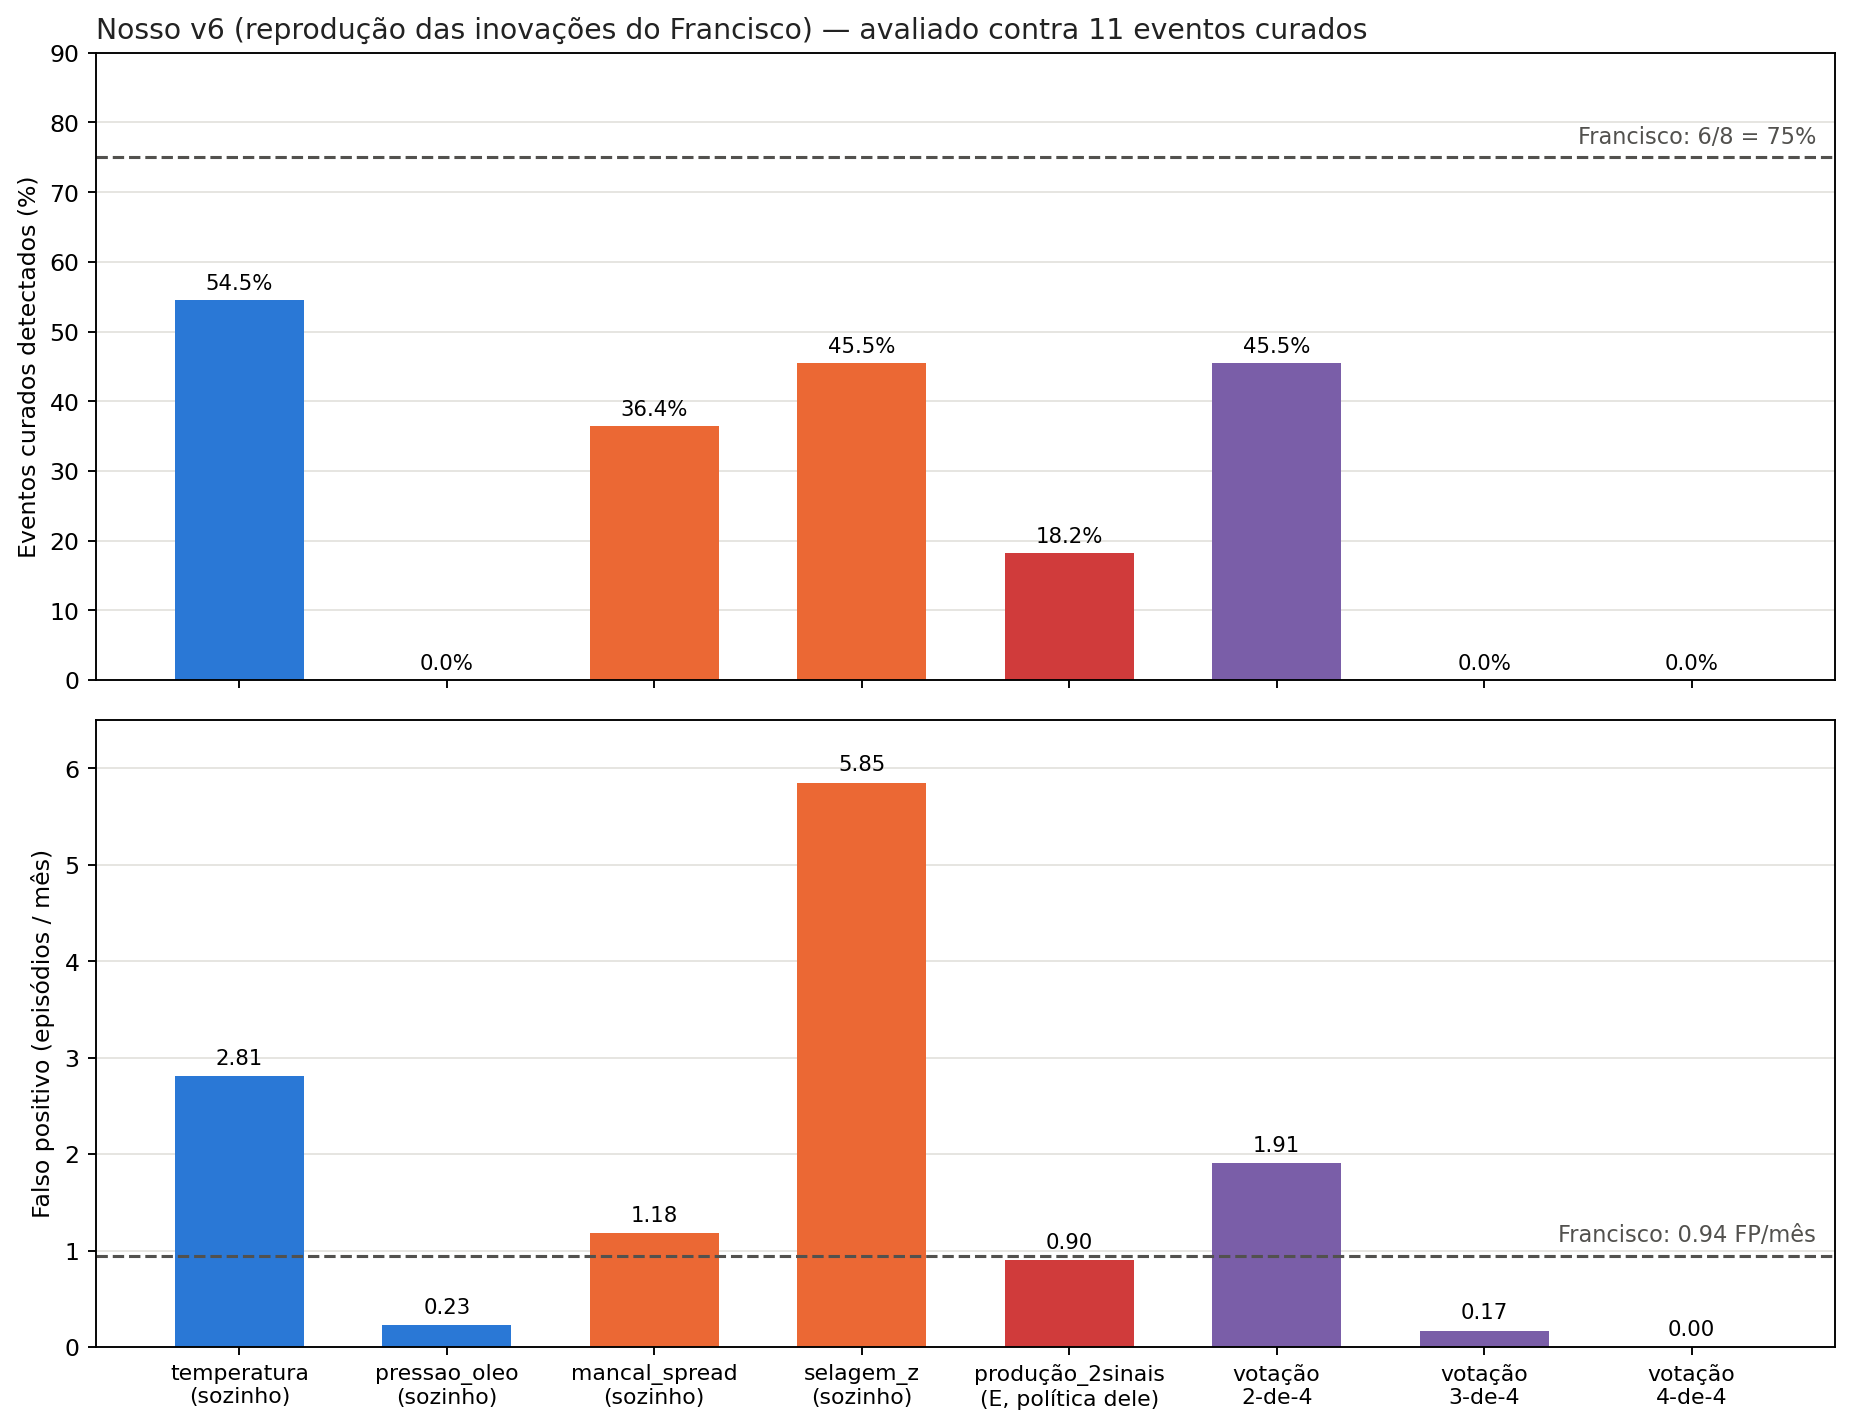
\includegraphics[width=0.95\textwidth]{fig_comparativo_sinais.png}
\caption{Cobertura de eventos e falso positivo por mês, por sinal e por
política de confirmação. A linha tracejada marca o resultado reportado
pelo Francisco (6/8 eventos, 0,94 FP/mês).}
\label{fig:comparativo}
\end{figure}

\subsection{O falso positivo foi replicado quase exatamente}

\begin{table}[H]
\centering
\begin{tabular}{@{}lccc@{}}
\toprule
& \textbf{Francisco} & \textbf{Nosso v6} & \textbf{Diferença} \\
\midrule
FP/mês (política de 2 sinais, E) & 0,94 & \textbf{0,90} & $-4,3\%$ \\
Eventos detectados & 6/8 (75\%) & 2/11 (18,2\%) & --- \\
Antecedência média & --- & 13,2h & --- \\
\bottomrule
\end{tabular}
\caption{Comparação direta entre o resultado documentado por ele e a
nossa reprodução do mesmo mecanismo (confirmação E entre 2 sinais
independentes), com \texttt{scikit-learn} puro sobre o nosso
pré-processamento.}
\label{tab:comparacao-principal}
\end{table}

A leitura central deste relatório: \textbf{a supressão de falso positivo
não vem de um modelo mais preciso ponto a ponto --- vem do mecanismo de
confirmação entre sinais independentes.} Isolado, o sinal
\texttt{temperatura} tem FP de 2,81/mês; isolado, \texttt{mancal\_spread}
tem 1,18/mês. Exigir que os dois concordem simultaneamente derruba o
conjunto para 0,90/mês --- um número quase idêntico ao dele, obtido com
uma implementação independente, em cima de um dataset diferente e um
ground-truth com mais que o dobro de eventos.

% Placeholder p/ os graficos de zoom -- inseridos apos a task v6b terminar
\subsection{Visão geral do período avaliado}

Antes do zoom por evento, a Figura~\ref{fig:serie-completa} mostra o
score de temperatura (máximo diário, escala log) ao longo dos 26 meses
avaliados, com os 11 eventos curados marcados (verde = detectado pela
política de 2 sinais, vermelho = não detectado) e os dias em que houve
pelo menos um alerta confirmado (E). Fica visível que o detector dispara
com alguma frequência fora dos eventos catalogados --- o que pode ser
tanto falso positivo genuíno quanto sinal de degradação real que nunca
chegou a virar parada catastrófica (não temos como distinguir os dois
sem uma auditoria manual, item já registrado nos próximos passos).

\begin{figure}[H]
\centering

\includegraphics[width=0.97\textwidth]{fig_serie_completa.png}
\caption{Score de temperatura ao longo de todo o período avaliado
(mar/2024--abr/2026), com os 11 eventos curados e os dias com alerta
confirmado (E) marcados.}
\label{fig:serie-completa}
\end{figure}

\subsection{Casos detectados (acertos)}
\label{sec:acertos}

As Figuras~\ref{fig:hit1} e~\ref{fig:hit2} mostram os dois eventos que a
política de 2 sinais conseguiu antecipar. Em ambos, o padrão é o mesmo:
o \texttt{mancal\_spread} fica elevado (acima de $|z|=3$) por um período
mais longo antes do evento, e a confirmação (E) fecha no instante em que
o score de \texttt{temperatura} também cruza seu limiar --- geralmente
numa janela curta de poucas horas, o que explica por que a antecedência
útil (12--14h) é bem menor que a janela em que o \texttt{mancal\_spread}
já estava sinalizando sozinho.

\begin{figure}[H]
\centering
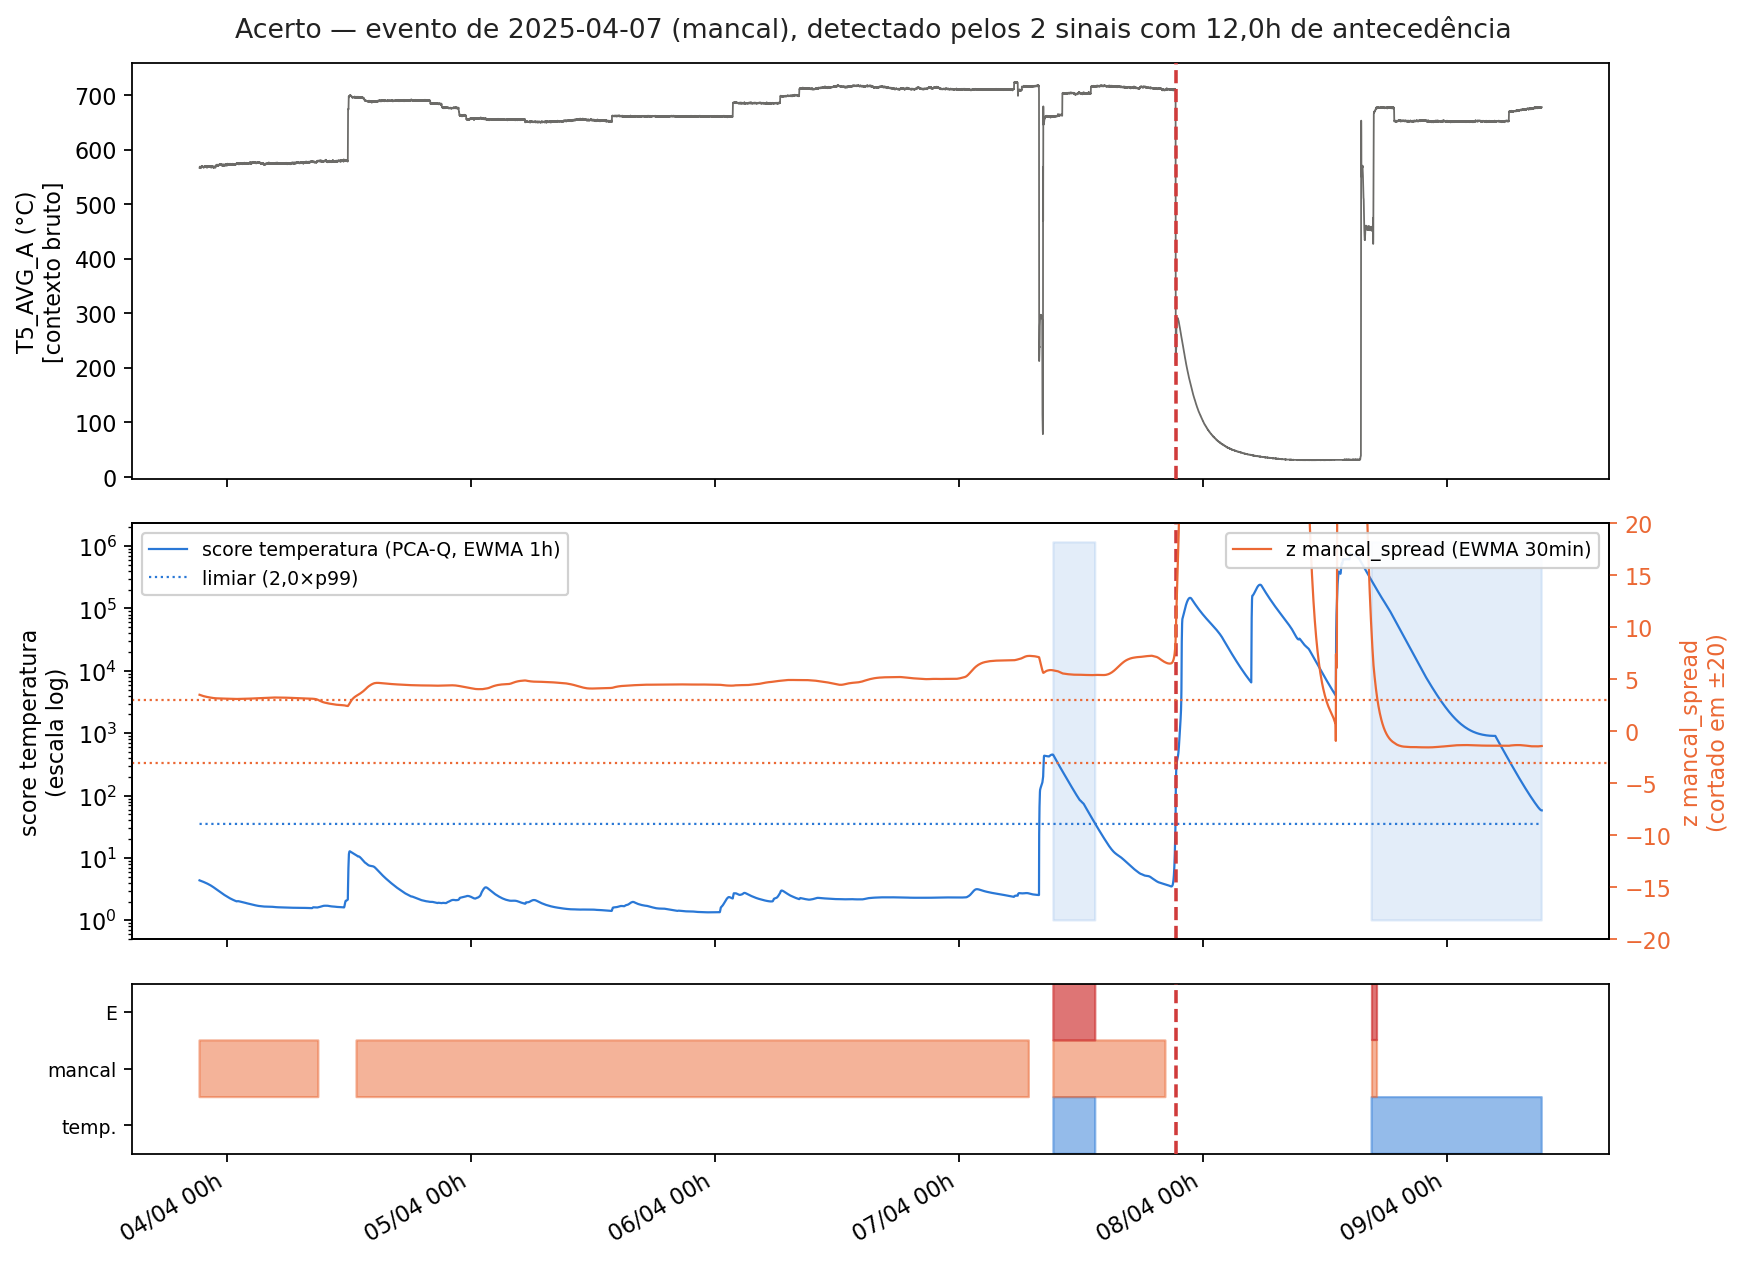
\includegraphics[width=0.95\textwidth]{fig_zoom_hit_2025-04-07.png}
\caption{Evento de 2025-04-07 (mecanismo de mancal): os dois sinais
concordam $\sim$12h antes da parada real (linha vermelha tracejada).}
\label{fig:hit1}
\end{figure}

\begin{figure}[H]
\centering
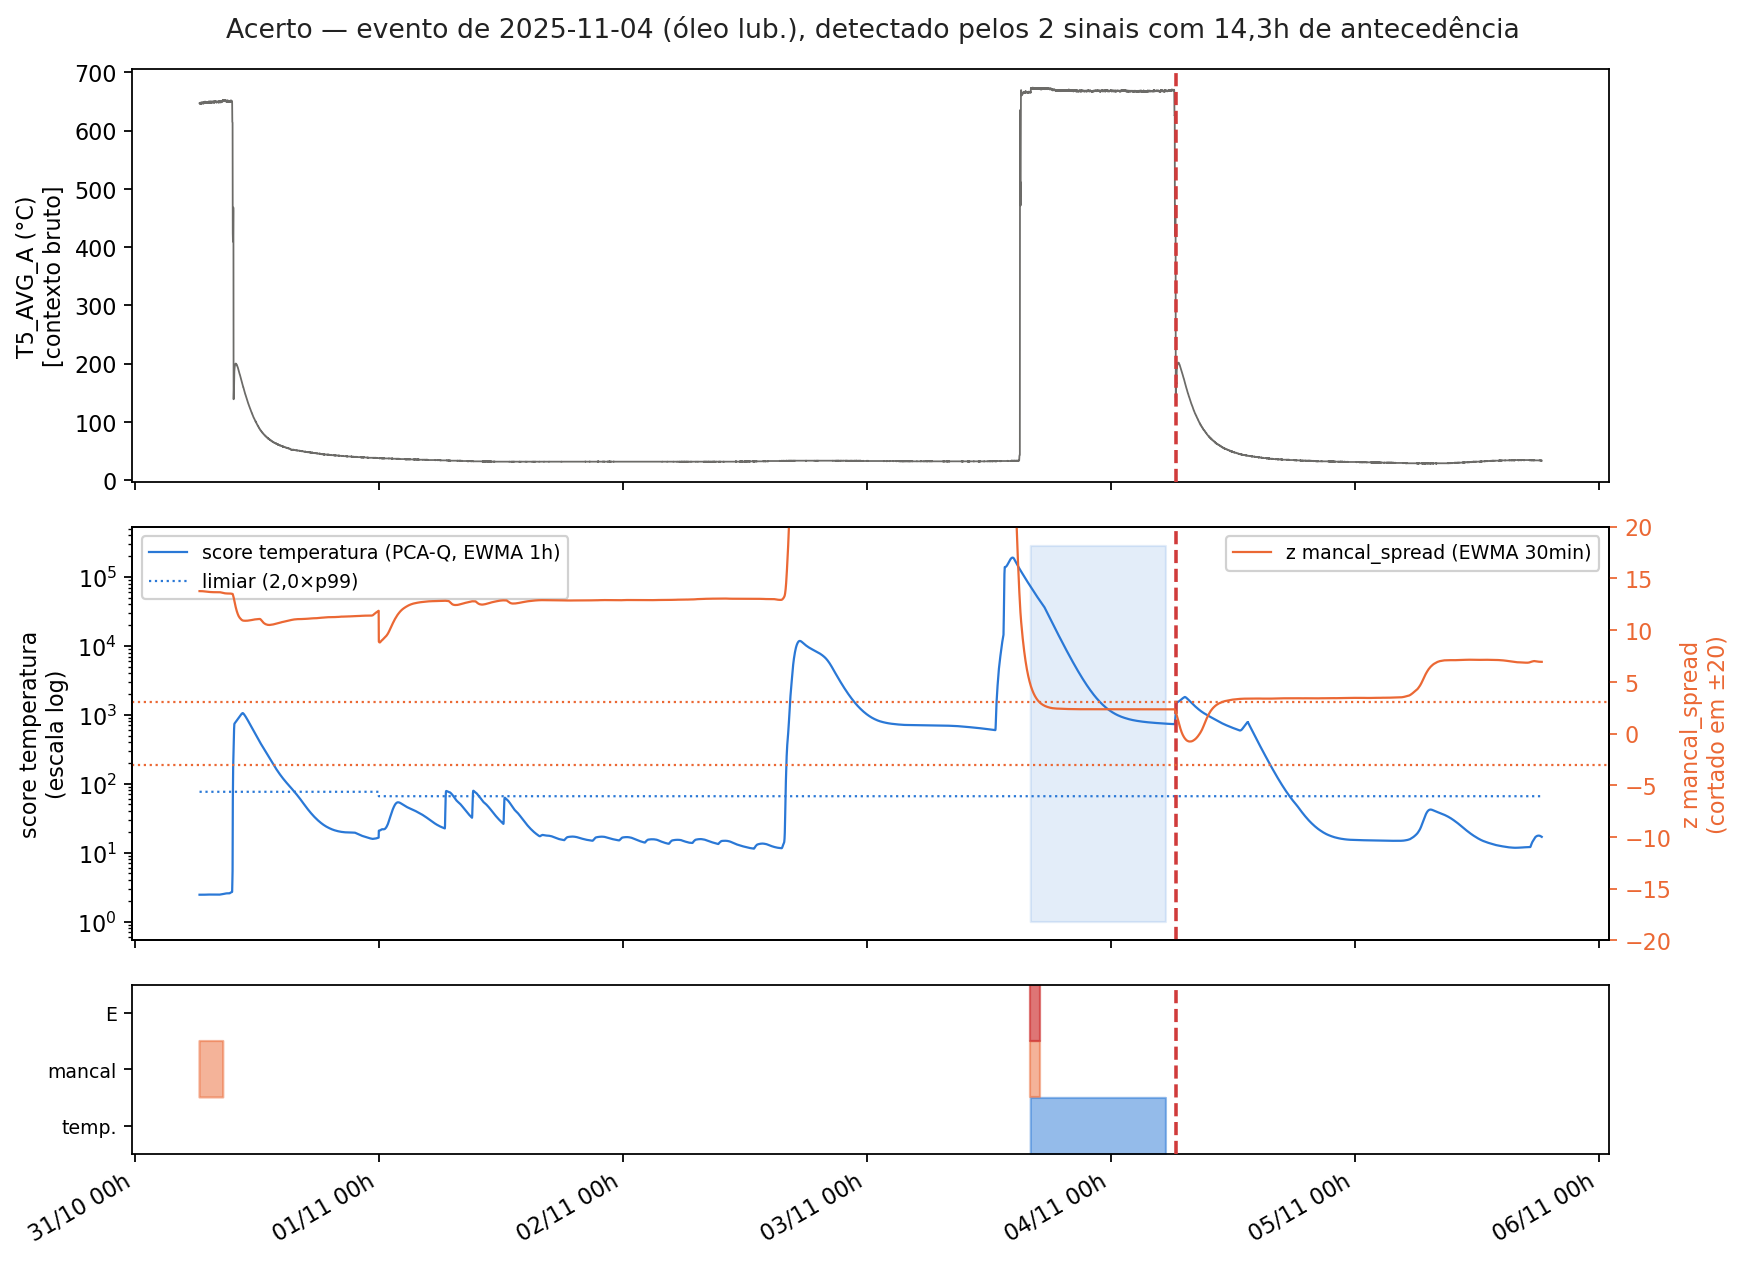
\includegraphics[width=0.95\textwidth]{fig_zoom_hit_2025-11-04.png}
\caption{Evento de 2025-11-04 (óleo lubrificante): os dois sinais
concordam $\sim$14h antes da parada real.}
\label{fig:hit2}
\end{figure}

\subsection{Casos não detectados (erros)}
\label{sec:erros}

As Figuras~\ref{fig:miss1} e~\ref{fig:miss2} ilustram os dois padrões de
erro mais comuns entre os 9 eventos não detectados pela política de 2
sinais.

\textbf{Padrão 1 --- sinais corretos, janelas desencontradas.} Na
Figura~\ref{fig:miss1} (evento de 2025-04-11), tanto
\texttt{temperatura} quanto \texttt{mancal\_spread} ultrapassam seus
limiares \emph{antes} do evento --- mas em momentos diferentes, sem
sobreposição simultânea suficiente para a confirmação E fechar dentro da
janela de detecção. É um "quase acerto": os dois sinais captaram alguma
coisa, mas não ao mesmo tempo.

\textbf{Padrão 2 --- sinal errado para o mecanismo de falha.} Na
Figura~\ref{fig:miss2} (evento de 2025-02-27, mecanismo de selagem), a
temperatura antecipa a falha com folga (33,7h), mas o
\texttt{mancal\_spread} permanece completamente estável --- fisicamente
esperado, já que uma falha de selagem não tem por que perturbar o
equilíbrio térmico entre mancais. Como a política de produção exige
\emph{especificamente} esses dois sinais, um evento cujo mecanismo não
afeta o mancal nunca vai fechar a confirmação, não importa quão claro o
sinal de temperatura seja.

\begin{figure}[H]
\centering
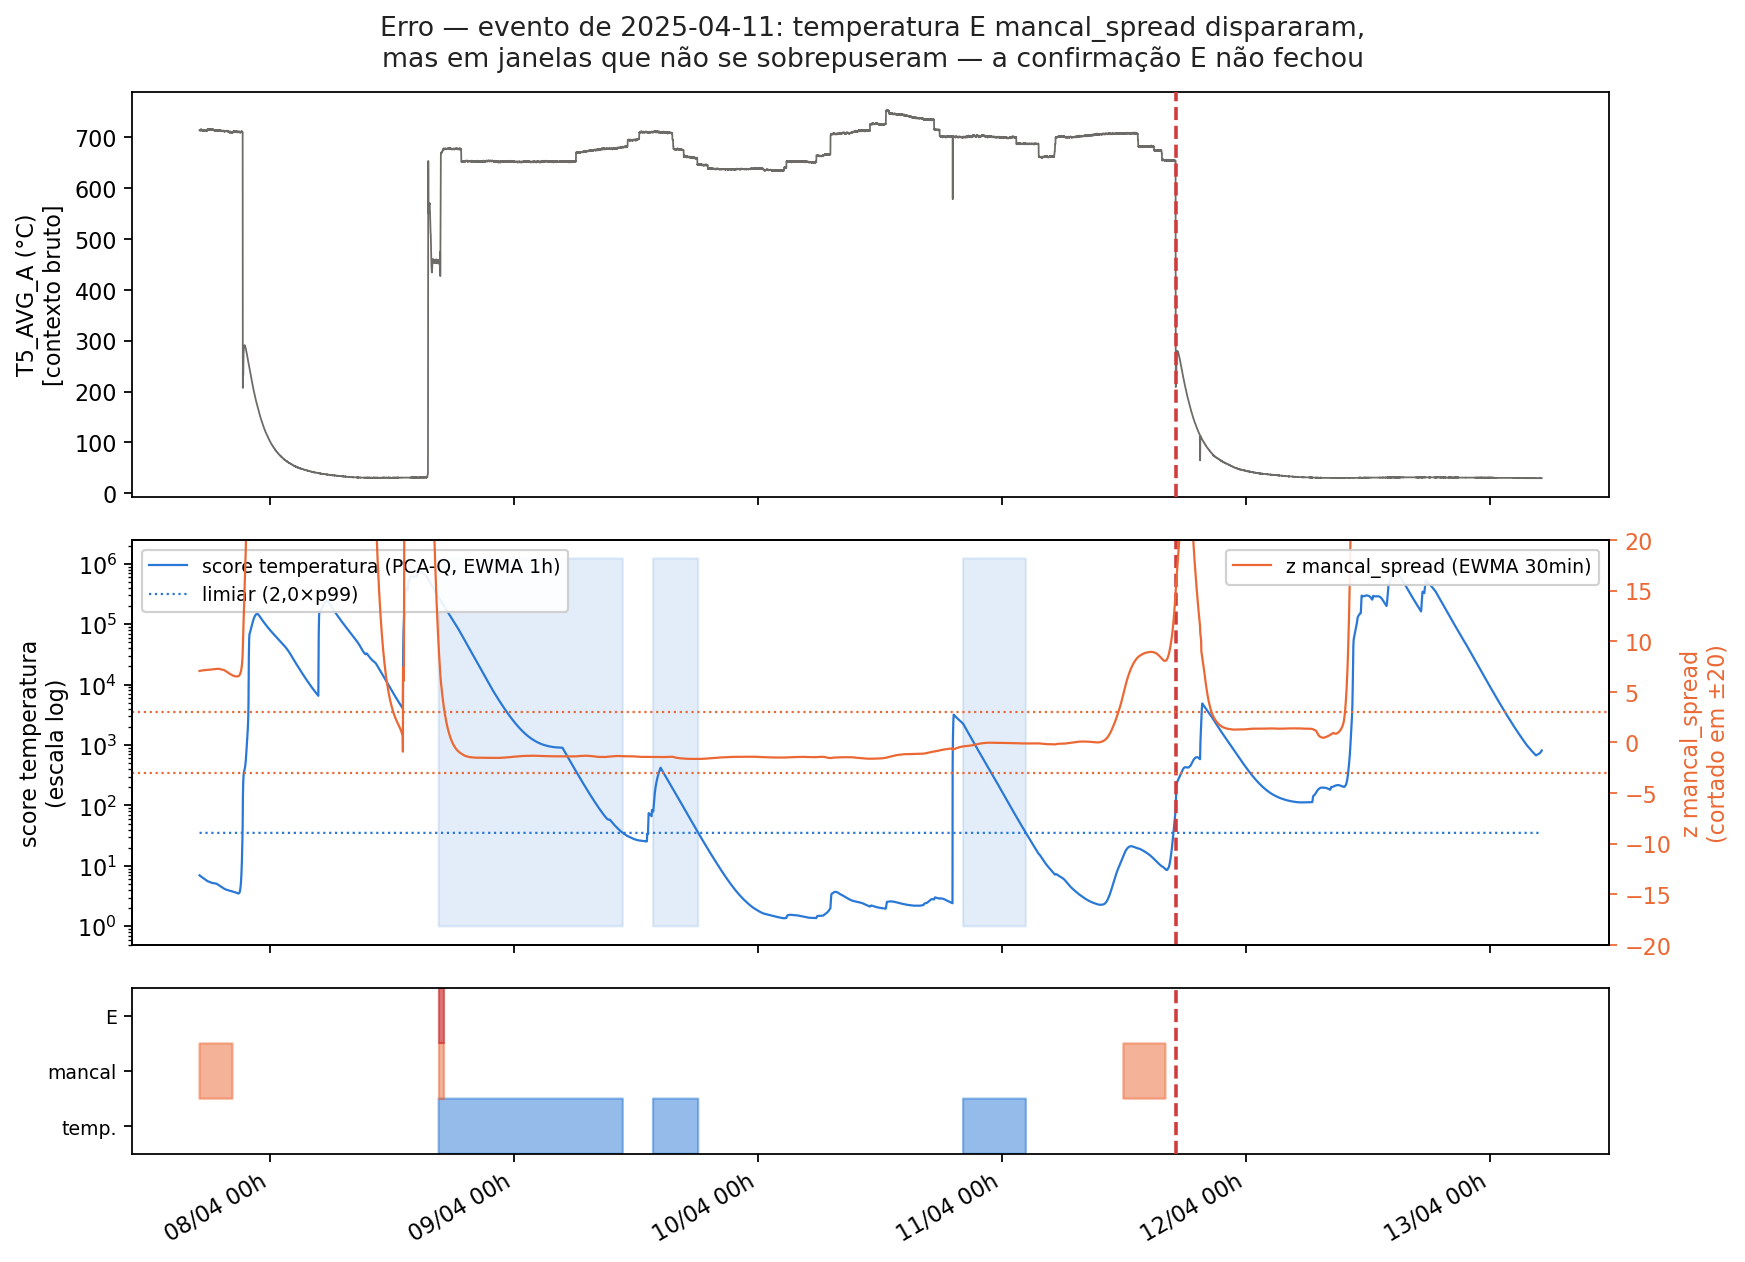
\includegraphics[width=0.95\textwidth]{fig_zoom_miss_2025-04-11.png}
\caption{Evento de 2025-04-11: os dois sinais dispararam, mas não
simultaneamente.}
\label{fig:miss1}
\end{figure}

\begin{figure}[H]
\centering
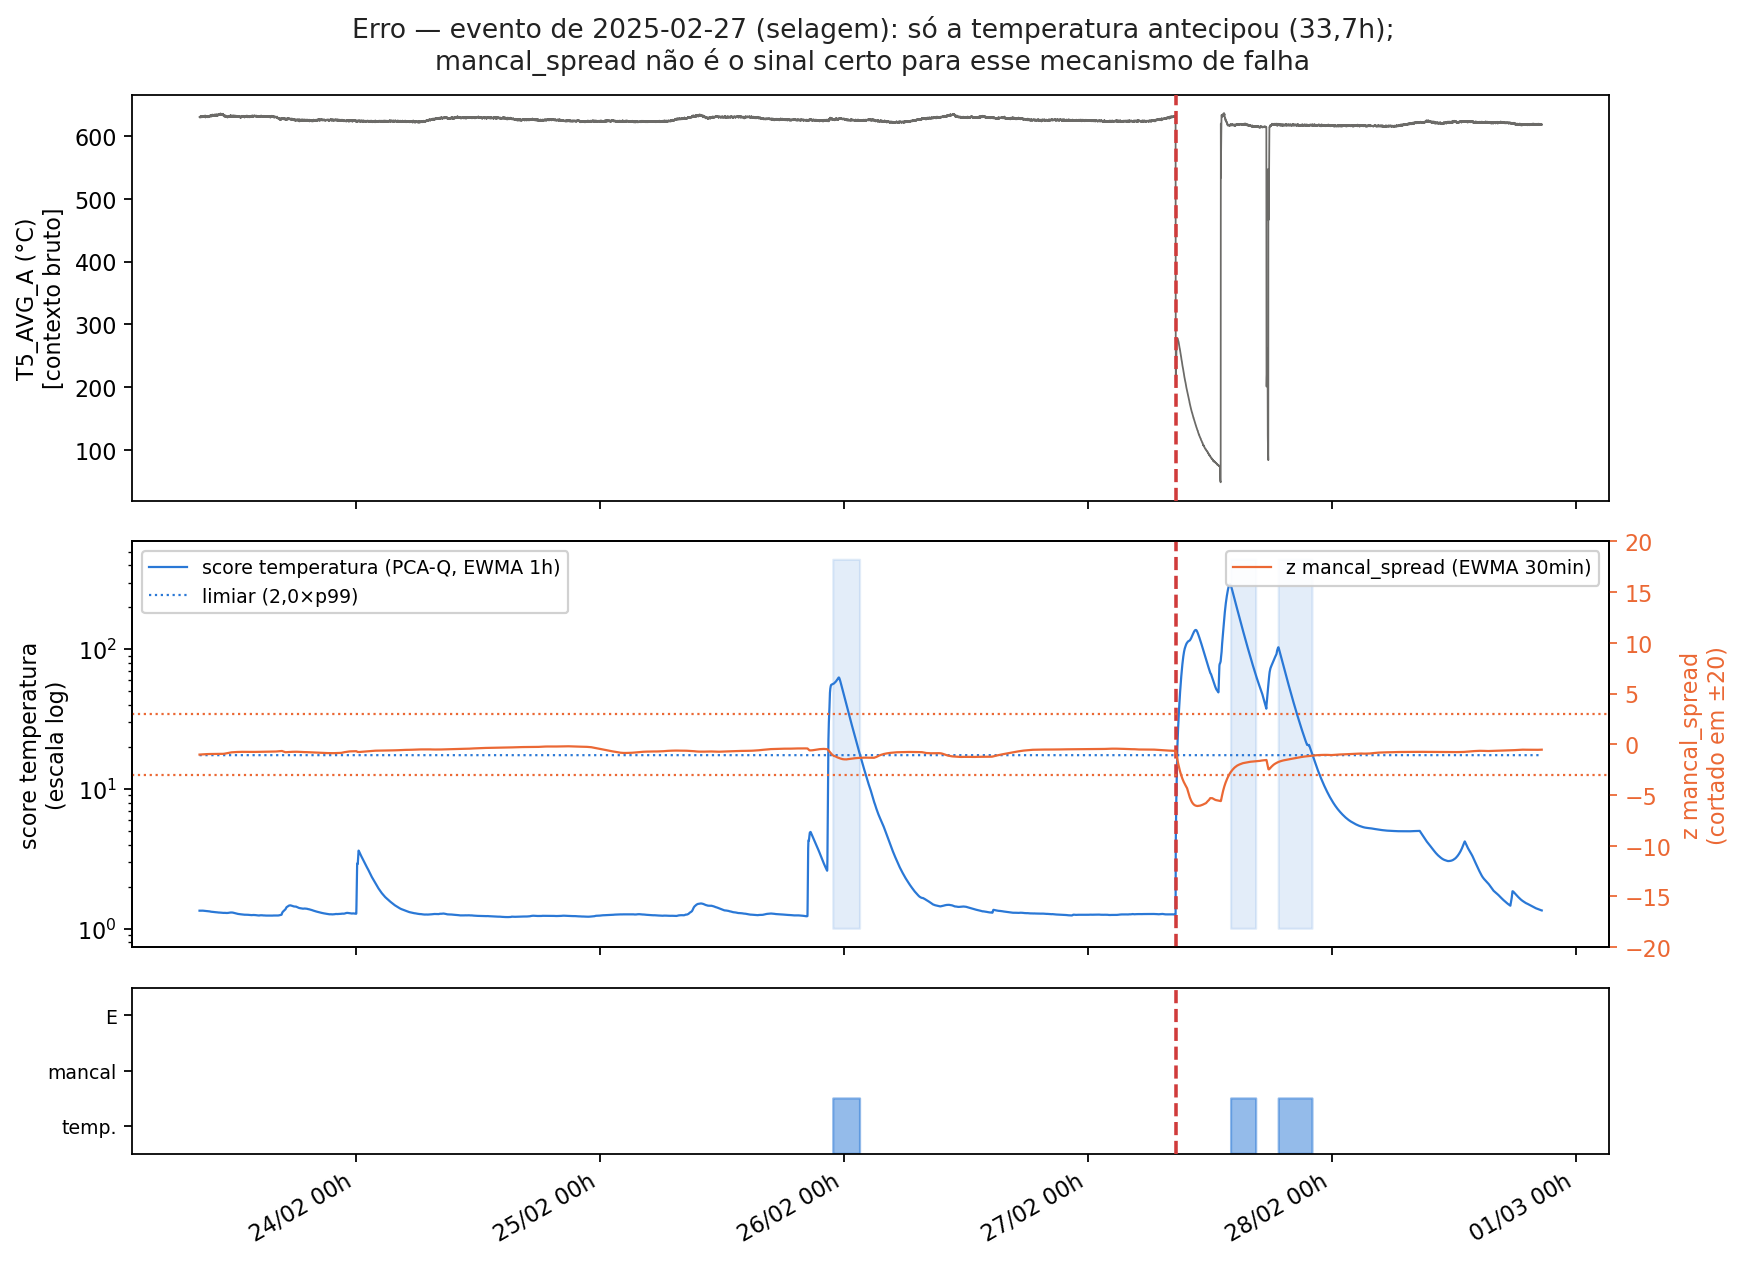
\includegraphics[width=0.95\textwidth]{fig_zoom_miss_2025-02-27.png}
\caption{Evento de 2025-02-27 (selagem): \texttt{mancal\_spread} não é o
sinal certo para este mecanismo de falha.}
\label{fig:miss2}
\end{figure}

% =====================================================================
\section{Interpretação e limitações}
\label{sec:interpretacao}
% =====================================================================

\begin{itemize}[leftmargin=1.4em]
  \item \textbf{O mecanismo de confirmação é a explicação principal do
  gap de FP} que vínhamos tentando explicar desde a Seção~\ref{sec:v3} ---
  não a janela de treino (testamos e refutamos essa hipótese no v3), nem
  o modelo em si (PCA-Q e PCA+\texttt{iforest} têm FP na mesma ordem de
  grandeza quando avaliados isoladamente).
  \item \textbf{A cobertura de eventos ainda não bate.} 2/11 contra 6/8
  é uma diferença grande demais para atribuir a acaso amostral. Hipótese
  mais provável, ainda não testada: nós rodamos o PCA-Q sobre o espaço
  de \textbf{features derivadas completo} do projeto ($\sim$196 colunas
  por família, com médias/desvios/tendências em 4 janelas), enquanto ele
  roda direto sobre os \textbf{14 sensores brutos} limpos. Um espaço de
  entrada de dimensão muito maior pode diluir o erro de reconstrução de
  um evento pontual de falha --- o oposto do problema de diluição que
  motivou os sinais \texttt{mancal\_spread}/\texttt{selagem\_z} em
  primeiro lugar, mas na mesma família de causa.
  \item \textbf{Vibração continua mal servida} em toda a série de
  experimentos (v1 a v6) --- reforça que ela é mais útil como
  \emph{feature} de contexto do que como alvo de predição direto,
  consistente com a decisão dele de colocá-la em quarentena.
  \item \textbf{Esta não é uma comparação 1:1 rigorosa.} Datasets,
  períodos avaliados, e vários hiperparâmetros de limpeza do baseline
  (\texttt{exclude\_days}, \texttt{exclude\_alarm\_h}) não são idênticos
  aos dele --- porque a grade completa de 31.104 configurações testadas
  por ele não está disponível para nós. O valor deste exercício é
  \emph{mecanístico}: confirmar que entendemos corretamente por que a
  arquitetura dele produz o número que produz, replicando o efeito
  principal (supressão de FP) de forma independente.
\end{itemize}

\subsection{Recapitulando o caminho até aqui}
\label{sec:v3}

Antes de investigar a branch dele, testamos e descartamos a hipótese
mais óbvia para o gap de FP: trocar a nossa janela de treino
\emph{expansiva} (todo o histórico anterior ao mês avaliado) por uma
janela \emph{rolante fixa} de $\sim$3000h corridas de calendário (v3).
O resultado foi o oposto do esperado --- o FP \textbf{piorou} (no
\texttt{ocsvm}, quase triplicou). Em retrospecto, agora sabemos por quê:
reproduzimos ``3000h'' de forma diferente da dele (calendário corrido, não
horas elegíveis --- Seção~\ref{sec:baseline-window}), então testamos uma
janela genuinamente mais curta em dado útil, que expôs o modelo a menos
variedade de operação normal. Corrigir isso é um próximo passo natural,
mas de prioridade menor que o gap de cobertura de eventos.

% =====================================================================
\section{Próximos passos}
% =====================================================================

\begin{enumerate}[leftmargin=1.6em]
  \item \textbf{[Prioridade alta]} Testar o sinal \texttt{temperatura}
  sem features derivadas (\texttt{ENABLE\_DERIVED\_FEATURES=False}), só
  sensor bruto limpo --- isolar se essa é a causa do gap de cobertura de
  eventos (Seção~\ref{sec:interpretacao}).
  \item Testar o limiar por k-ésimo-maior (Seção~4.6 do levantamento da
  branch dele) como alternativa ao percentil.
  \item Testar a janela de baseline em horas \emph{elegíveis} (não
  calendário) na nossa pipeline v2/v4 original (PCA+\texttt{iforest}
  sobre todos os sensores), já que o v3 tinha reproduzido isso errado.
  \item Auditar manualmente os 9 eventos não detectados pela política de
  2 sinais, caso a caso, para entender se algum subconjunto tem
  precursor físico não capturado por nenhum dos 4 sinais atuais (mesma
  disciplina do EXP16).
  \item Conversar com o Francisco sobre os hiperparâmetros de limpeza do
  baseline (\texttt{exclude\_days}/\texttt{exclude\_alarm\_h}) que não
  conseguimos inferir só pela leitura do código.
\end{enumerate}

\end{document}
